\chapter{Tools for Constructing and Testing Neuromechanical Models}\label{ch:sns}
\graphicspath{{../Figures/60-sns/}{figs/60-sns/}}
\edef\snsSavedWidowPenalty{\the\widowpenalty}
\edef\snsSavedClubPenalty{\the\clubpenalty}
\widowpenalty=10000\clubpenalty=10000

A neuromechanical simulation couples a neural controller to a mechanical model of the body it controls. Motor-neuron activity recruits actuators, the resulting forces move or load the joints, and sensory pathways carry measurements of that response back to the controller. I wanted to transfer a locomotor circuit from one model of the legs to another. A circuit that alternates the legs in suspension must also coordinate muscle force with foot contact if the model is to support weight. I developed tools to inspect that loop one connection at a time and to repeat a mechanical test after changing a connection.

\section{The Controller-Transfer Problem}\label{sec:prior_walker}\label{sec:animatlab_results}\label{sec:sns_gaps}

The starting point was a controller-development project in AnimatLab. Changes in muscle attachment, joint motion, and inertia alter the movement produced by a given motor command. The same motion can also stretch different muscles in two models and return a different pattern of sensory activity. These effects tie the choice of controller to the body on which it is tested.

For a course project in neuromechanical modeling, Morrow and I coupled the sagittal-plane biped of \citet{li_bipedal_2017} to the two-level central pattern generator (CPG) of \citet{deng_neuromechanical_2019} in AnimatLab \citep{cofer_animatlab_2010}. A shared rhythm generator (RG) drove pattern-formation (PF) pathways and motor neurons (MNs) on both sides. Antagonist Hill-type muscles acted on the thighs, shanks, and feet. I added a passive toe joint. We adjusted currents, synaptic weights, and muscle parameters by hand. Hunt and I reported the suspended model in a poster for the NIH BRAIN Initiative Investigators Meeting \citep{bolenTorqueValuesArtificialKnee2021June15-17}. Its legs cycled in suspension and the model tipped when released toward the ground (Figure~\ref{fig:animatlab_model_architecture}).

\begin{figure}[htbp]
\centering
\begin{minipage}[c]{0.46\textwidth}\centering
\textbf{(A)}\\[2pt]
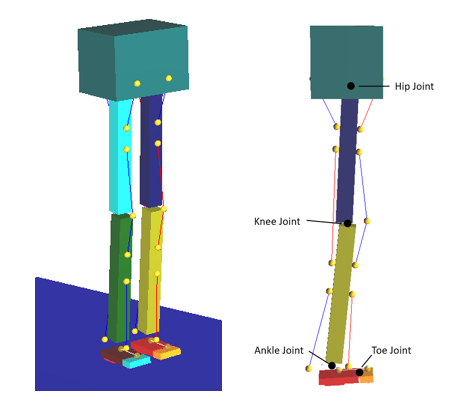
\includegraphics[trim=0bp 0bp 176.275bp 0bp,clip,width=\linewidth,height=0.19\textheight,keepaspectratio]{OurWalker.png}
\end{minipage}\hfill
\begin{minipage}[c]{0.46\textwidth}\centering
\textbf{(B)}\\[2pt]
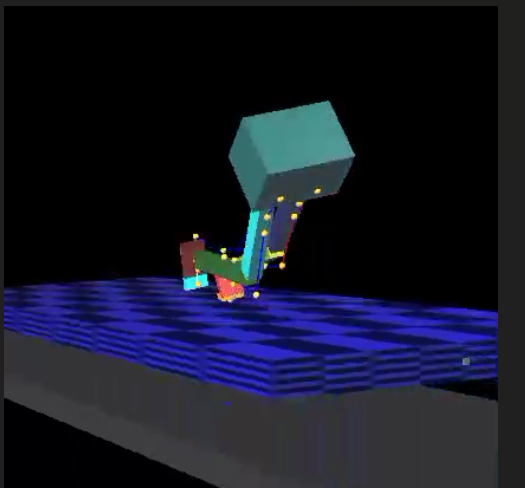
\includegraphics[width=\linewidth,height=0.19\textheight,keepaspectratio]{LI_DENG_FALL_FRAME.png}
\end{minipage}
\caption[Original controller-transfer experiment]{The AnimatLab walker assembled by Morrow and Bolen cycled its legs in suspension (A) and tipped when released for the ground test (B).}
\label{fig:animatlab_model_architecture}
\end{figure}

The fall left us with a practical diagnostic problem. An extensor might have received its command too late, produced too little force, or acted through an unsuitable moment arm. Watching the legs or retuning all three together could not distinguish those explanations. I needed to record a command, its force, the resulting joint motion, and the sensory current returned to the circuit on a common clock.

I built on OpenSim, MyoConverter, MuJoCo, SNS-Toolbox, Simulink, and Simscape \citep{delp_opensim_2007,caggiano_myosuite_2022,todorov_mujoco_2012,nourse_sns_2023}. My contribution was to prepare mechanical models, implement editable neural and actuator blocks, connect neural outputs with actuator commands and mechanical measurements with sensory inputs, and write drivers that repeat interventions with a saved controller. The methods below describe how to assemble an experiment. The results start with a single joint, then examine how sensory return and mechanical assistance change bilateral coordination. Appendix~\ref{app:simulation_verification} gives the executable examples and scoring definitions.

\section{Methods for Constructing and Testing a Coupled Model}\label{sec:preliminary_sim_methods}

\subsection{Workflow and Experimental Models}\label{sec:sns_existing_tools}\label{sec:sns_gait_comparison_main}

To test a pathway, first choose a mechanical model and identify what its actuators can apply and its sensors can measure (Figure~\ref{fig:simulation_workflow}). Then specify the neural calculation and the physical condition under which its effect should be observable. For example, a sensory current applied to the extensor pathway of a loaded knee should change MN activity before it changes knee angle. A recording of both signals tests that sequence.

\begin{figure}[!htbp]
\centering
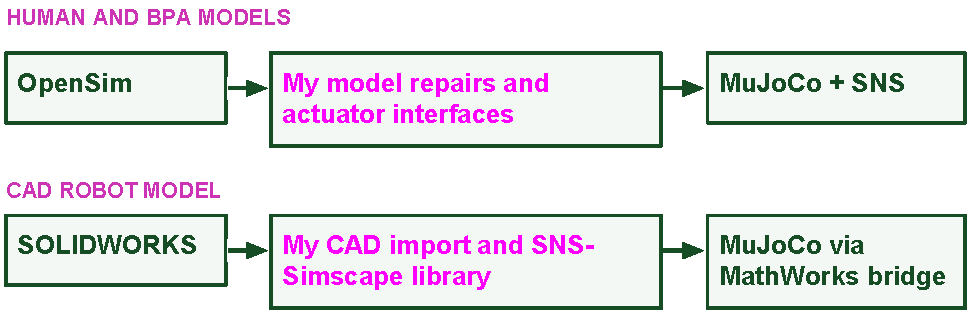
\includegraphics[width=14cm]{simulation_workflow_authoritative.pdf}
\caption[Workflow for neuromechanical model construction and testing]{Mechanical preparation supplies an executable model. Neural commands pass through the actuator interface to generate force, while mechanical measurements return through sensory encoding. Functional calibration, physical tests, and aligned recordings support inspection of the coupled response.}
\label{fig:simulation_workflow}
\end{figure}

I used two routes to prepare the mechanics. For imported musculoskeletal models, I converted OpenSim geometry and muscle paths with MyoConverter and checked the result in MuJoCo. For CAD assemblies, I used joint frames, inertial properties, and attachments to assemble mechanisms for Simscape Multibody or, separately, MuJoCo. A researcher can also run a Simulink controller against existing MuJoCo mechanics through the runtime bridge. That route exchanges commands and measurements at each update and requires an executable MuJoCo model.

\noindent\begin{minipage}{\linewidth}Table~\ref{tab:sns_model_configurations} identifies the body and force law used in each experiment. The original shared-RG walker, the later bilateral W2L controllers, and the separately assembled CAD robot answer different transfer questions. BiW2Lvar+ denotes an expanded graded controller used on the Gait2392 human model. Its software selector is \texttt{hunt}.

\begin{table}[H]
\centering\small
\caption[Mechanical models and actuators]{Mechanical models, actuator formulations, and the experiments for which they were used.}
\label{tab:sns_model_configurations}
\begin{tabularx}{\textwidth}{@{}>{\raggedright\arraybackslash}p{0.23\textwidth}>{\raggedright\arraybackslash}p{0.31\textwidth}>{\raggedright\arraybackslash}X@{}}
\toprule
Mechanical model & Actuation and controller & Experimental use \\
\midrule
Single-joint knee and arm & Antagonist reflex circuits with simplified knee actuators or BPA20 arm actuators & Pulse the knee sensory current or raise the load in the cup. \\
Li--Deng and W2L walkers & Shared RG in the original transfer, bilateral controllers in later W2L models & Compare suspended and released motion, then test contact coordination on a supported treadmill. \\
Gait2392 human & Biological muscles driven by named graded or spiking controllers & Compare forces at matched poses and evaluate each controller in its specified physical task. \\
Gait2392 robot counterpart & Robot-specific paths with selectable muscle or BPA force laws & Test a change of force law on the routed robot. Suspended cycling used Hill-type muscles. \\
CAD robot & SNS timing and engineering allocation to 54 ideal tension actuators & Test contact handover and swing clearance under measured assistance. \\
\bottomrule
\end{tabularx}
\end{table}\end{minipage}

\noindent\begin{minipage}{\linewidth}Table~\ref{tab:sns_capability} gives a starting point for each type of experiment. The graphical tools expose individual connections and their signs. The scripts run the same circuit and intervention repeatedly without a graphical interface. A saved set of parameters and a recording link a result to the controller that produced it.

\begin{table}[H]
\centering\small
\caption[Tools developed or adapted for controller experiments]{Tools I developed or adapted, their inputs, and the measurements used to test them. Appendix~\ref{sec:app_execution_provenance} gives their repository locations.}
\label{tab:sns_capability}
\begin{tabularx}{\textwidth}{@{}>{\raggedright\arraybackslash}p{0.35\textwidth}>{\raggedright\arraybackslash}X@{}}
\toprule
Tool or adaptation & Researcher's action and verification \\
\midrule
Mechanical preparation scripts & Build robot-specific paths with \path{repair_robotbody_muscles.py}, then inspect joint action and force at matched poses. On the CAD model, check path derivatives against virtual work. \\
SNS-Simscape block library and \texttt{SNSGui} & Wire a graded circuit in the editor and build it with \path{sns_build_from_json.m}. Run the separate coupled knee example to measure sensory-current transmission. \\
Actuator and sensor interfaces & Select a muscle law and map MN output to activation or pressure. The adapted MuJoCo--Simulink bridge returns joint and actuator measurements for comparison with Python readback. \\
Calibration and intervention scripts & Specify a recruitment or timing target, fit a circuit, and replay the saved candidate. Compare intact and perturbed trials at the same drive and mechanical support. \\
Sparse neural execution and recording & Run the reference and accelerated backends on the same inputs. Compare the recorded neural and mechanical arrays before comparing elapsed times. \\
\bottomrule
\end{tabularx}
\end{table}\end{minipage}

\subsection{Preparing the Mechanical Models}\label{sec:sns_cad_methods}

For the human-model route, I converted the Gait2392 reference from OpenSim to MuJoCo with MyoConverter. The robot counterpart required separate preparation because its artificial-muscle routes could not be combined with unchanged human-muscle parameters. Biological-muscle actuators were retained in the human reference, while robot routes and BPA forces were handled through explicit interfaces. The human model retains 92 actuator entries; six small hip-rotator entries remain disabled. The knee retains OpenSim's flexion-negative convention.

I checked individual actuators before fitting the controller. A pull on one muscle reveals its direction of action. Moving a joint through its range reveals whether a path point or wrap surface changes the moment arm as intended. Foot contact forces distinguish load transmitted through the sole from unintended collisions elsewhere on the model. Appendix~\ref{sec:app_conversion_repairs} describes the repairs and the muscles with remaining force discrepancies.

The CAD route additionally required consistent anatomical frames, mass and inertia assignment, joint topology, and actuator attachments. The robot frame uses $x$ anterior, $y$ superior, and $z$ right. CAD assembly placement was related to that frame through a reference datum. The four-bar knees require their loop constraints to be retained in the dynamic model. Moving and conditional muscle-route points require both geometric updates and the corresponding force derivatives; changing a route's length without accounting for that dependence would give inconsistent generalized forces. Numerical derivative and virtual-work checks test those relations before interpreting motion.

For BPA actuation, my interface evaluates the quasi-static force law from Chapter~\ref{ch:muscles} at the current routed length and commanded pressure and applies tensile force along the route. This allows a researcher to change the force law while retaining the mechanical geometry. The calculation assumes that commanded pressure is available at the actuator. Valve filling and loading-history effects require separate measurements.

\subsection{Constructing Controllers and Closing the Feedback Loop}\label{sec:sns_new_tools}\label{sec:w2l_matlab_attempt}\label{sec:sns_bridge_methods}

I implemented the SNS-Simscape library as editable Simulink blocks for neurons, synapses, sensory encoding, activation, and actuator force (Figure~\ref{fig:simulink_sns_implementation}). The graded equations follow SNS-Toolbox \citep{nourse_sns_2023}. Each synapse sends a conductance and its product with reversal potential to the postsynaptic neuron. This makes the sign and strength of a connection available for inspection. From the \path{Code/Matlab/SNS_Simscape/gui} directory, running \verb|app = SNSGui()| opens my circuit editor. A user can place and connect graded neurons, save the circuit description, and generate a Simulink circuit through \path{sns_build_from_json.m}. Separate builders connect complete reflex circuits to the knee and arm dynamics.

\begin{figure}[!htbp]
\centering
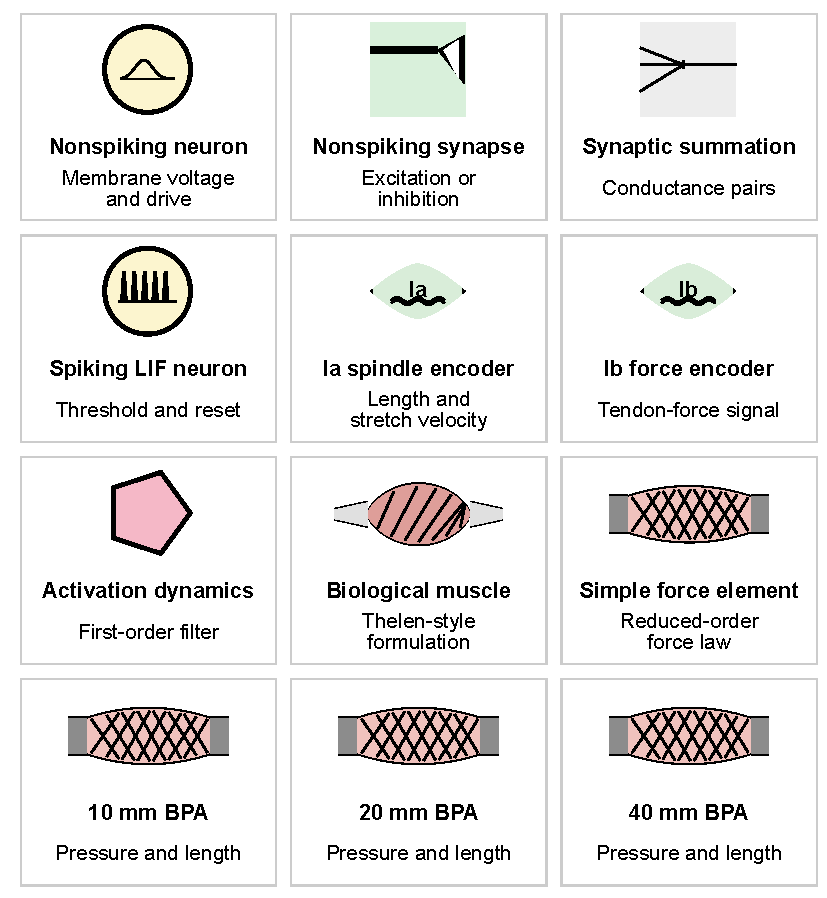
\includegraphics[width=14cm]{sns_library_20261116.pdf}
\caption[Editable SNS-Simscape blocks]{The twelve SNS-Simscape library elements for constructing neural pathways, encoding sensory measurements, and calculating activation and actuator force. The editable blocks connect these operations through stated signal interfaces.}
\label{fig:simulink_sns_implementation}
\end{figure}

In the reduced knee, extensor and flexor MN outputs pass through activation dynamics to antagonist tensile actuators. Their moments change the knee angle and angular velocity. The spindle-like transducers use joint motion to produce Ia currents, and the Ib transducers use actuator tension. Each Ia pathway excites its own MN and inhibits the antagonist. Each Ib pathway inhibits its own MN. The resulting six connections close the loop that the worked example tests. The Gait2392 and W2L experiments use different sensory encoders and input ports, identified in Appendix~\ref{sec:app_signal_contracts}.

SADb links a candidate feedback pathway to the experiment that motivated it (Chapter~\ref{ch:database}). To implement a pathway, I specify the measured quantity, the sign of the connection, its operating range, and its target population. Stimulating a sensory input to an MN tests recruitment. A projection to the PF or RG layer can also alter the timing of later recruitment.

For experiments with MuJoCo mechanics, I integrated the blocks with the MathWorks MuJoCo--Simulink bridge and adapted initialization and sensor readback. A Simulink controller sends an ordered actuator-command array to MuJoCo and reads the resulting joint and actuator measurements. I tested a command source updated every \qty{1}{\milli\second} with a mechanical and sensor update every \qty{5}{\milli\second}. The separate Gait2392 neural and mechanical experiments used \qty{2}{\milli\second} updates.

\subsection{Functional Design, Neural Calibration, and Physical Curriculum}\label{sec:sns_curriculum_main}\label{sec:sns_literature_methods}

I specify the function of a neural pathway before fitting it. For a PF channel, the target includes the part of the cycle during which the channel should drive its MNs, the duration of that drive, and its overlap with neighboring channels. The test therefore examines the activity transmitted through its synapse. Voltage below the synapse's operating range can vary without changing motor recruitment. Appendix~\ref{app:neuron_equations} describes the graded and spiking formulations.

I adapted the four calibration operations presented by \citet{hunt_inrc_2019}. I set the intrinsic period to approximately twice the target locomotor period, tuned entrainment under expected afferent input, fitted feedforward motor recruitment, and refined the pattern with sensory feedback. The recruitment targets came from inverse mechanics applied to reference motion. Agreement with those targets measures how well the network reproduces the estimated activation pattern.

My physical test sequence changes the loads and sensory information available to the same candidate (Table~\ref{tab:sns_curriculum}). In air, a researcher can tune recruitment and timing before foot contact introduces another source of feedback. Standing and supported stepping then test whether the model carries load and transfers it between its feet. The evaluation scripts reload the saved candidate for each condition.

\begin{table}[htbp]
\centering\small
\caption[Physical curriculum for coupled-model evaluation]{Physical curriculum and task-specific observations. The stages define an evaluation sequence; they do not imply that every controller has completed the sequence.}
\label{tab:sns_curriculum}
\begin{tabularx}{\textwidth}{@{}c>{\raggedright\arraybackslash}p{0.29\textwidth}>{\raggedright\arraybackslash}X@{}}
\toprule
Stage & Physical condition & Principal observations \\
\midrule
1 & Deafferented air motion & Suspended rhythmic movement with sensory return disabled \\
2 & Afferented air motion & Rhythmic movement with stated sensory return and command conditions \\
3 & Standing & Posture and response to mechanical perturbation \\
4 & Supported ground stepping & Alternating loading, unloaded swing clearance, knee bounds, and measured assistance \\
5 & Contact refinement and reduced assistance & Timing and kinematics under declared contact pathways and loading demands \\
\bottomrule
\end{tabularx}
\end{table}

A result advances a particular controller and mechanical model. A good fit to an MN target can coexist with a timing error upstream, and suspended joint motion can coexist with poor weight transfer. I therefore tested the PF signals before interpreting a motor fit and tested foot loading separately from joint cycling.

\subsection{Automated Execution and Experimental Protocols}\label{sec:sns_repeatability_main}\label{sec:sns_w2l_methods}

For repeated searches I used bounded parameters, tied left and right homologues where symmetry was intended, and used tree-structured Parzen estimation to select candidates. The scripts save parameters, objective components, and the termination condition. A promising candidate is rerun in a fresh process with its fitted parameters before an intervention is introduced.

Acceptance begins with finite states, completion of the prescribed duration, and protected joint bounds. Suspended experiments assess meaningful joint excursion, cadence, and bilateral phase. Ground tests additionally require unloading, whole-foot clearance, contralateral loading, and a minimum interval duration specified for the model. Appendix~\ref{app:simulation_verification} gives the force, clearance, and duration thresholds for each contact test. Assistance is calculated from recorded forces over a declared window. Vertical lift, horizontal guidance, and attitude restraint are reported separately because reducing one does not remove the others. A nominal support setting is therefore insufficient to characterize the loading experienced by the model.

For a pathway removal, I retained the unaffected controller parameters, drive, support, and external force protocol. For a stimulation experiment, I changed the injected current at one location and compared it with an unperturbed run from the same state. Aligning RG, PF, and MN voltages with joint motion, actuator force, and support force identifies where the two runs first diverge.

I compared numerical trajectories before timing the neural backends. I measured the neural-update calls separately from the surrounding simulation because initialization, mechanics, and recording also consume time. The timed workloads and their reference implementations are specified with the results.

\section{Results of Controller and Mechanical Tests}\label{sec:preliminary_sim_results}

\subsection{Mechanical and Signal-Interface Verification}\label{sec:crossengine_results}

At matched poses and OpenSim static-optimization activations, eight of twelve sampled muscles gave force-prediction $R^2$ values of 0.87--0.98 and mean forces within \qty{10}{\percent} of the reference (Table~\ref{tab:force-r2}). Rectus femoris and biceps femoris short head had negative $R^2$. For those muscles, the mean reference force predicted the sampled force better than the converted model did. This comparison prescribed a pose and activation for each frame. Movement velocity and tendon dynamics were outside its scope.

The bridge delivered the prescribed muscle commands from Simulink to MuJoCo. All five tested sensor arrays matched Python readback bit for bit over 80 steps from \qty{0.005}{\second} through \qty{0.400}{\second}. An exported neural circuit drove all 92 actuator channels for \qty{5}{\second}. A separate reflex test returned mechanical measurements to the controller. Its length encoder saturated after initialization, so the experiment demonstrates bidirectional signal exchange while leaving sensitivity to length untested (Appendix~\ref{sec:app_signal_contracts}).

A successful interface still leaves a question about the circuit it carries. Under constant drive, one Simulink realization settled to a steady voltage while its NumPy reference oscillated. A larger export matched the early transient and diverged later. Comparing neural traces under common inputs localized these discrepancies before the mechanics complicated their interpretation (Appendix~\ref{sec:sns_ports}).

\subsection{Matched Circuit Calculations and Reflex Responses}\label{sec:sns_simulink_demos}

A contact-driven W2L test compared a 26-neuron Simulink rhythm core with the corresponding four RG signals in the 95-neuron NumPy network. With identical drive and prescribed heel inputs, both produced all ten expected bursts with a \qty{1.000}{\second} period over \qtyrange{2}{12}{\second}. The four best-lag voltage correlations were at least 0.99996 with a \qty{2}{\milli\second} relative alignment (Figure~\ref{fig:w2l_crossengine}). Removing phasic heel input caused both circuits to latch. The comparison verifies the shared rhythm-generating pathways under this stimulus.

A researcher can reproduce the knee experiment with \path{run_transient.m} and the archived \texttt{KneeReflexDemo} model. The driver runs the settled knee twice and adds a \qty{2}{\nano\ampere}, \qty{30}{\milli\second} pulse to the extensor Ia current in one run. The pulse recruited the extensor MN. The flexor was already inactive, so the rise in extensor force accounted for the initial extension (Figure~\ref{fig:sns_reflex_current}). The stimulated knee extended \ang{1.09} relative to the control, peaked \qty{111}{\milli\second} after pulse onset, and met the angle and speed recovery criteria \qty{6.355}{\second} after onset. Broader MN and Ia synaptic operating ranges allowed the model to settle before the pulse. The original narrow ranges produced sustained oscillation. Appendix~\ref{sec:app_knee_transient} gives the MATLAB command and the fields to inspect in the saved summary.

\begin{figure}[!htbp]
\centering
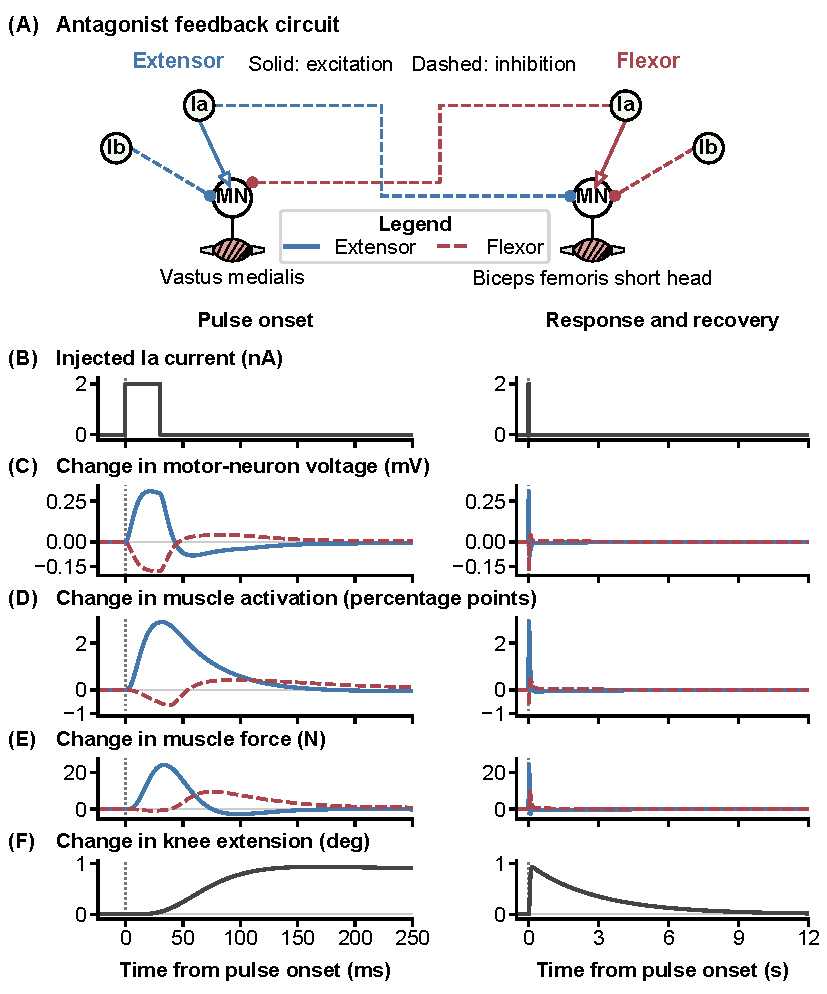
\includegraphics[width=14cm]{sns_knee_reflex_authoritative.pdf}
\caption[Transient knee feedback response]{Six feedback connections (A), sensory-current pulse (B), knee response (C), and MN activity (D). Panel B enlarges the pulse interval; C and D show the longer recovery. The \qty{2}{\nano\ampere}, \qty{30}{\milli\second} pulse follows settling. This test uses simplified linear actuation and broadened synaptic saturation ramps; flexion is negative.}
\label{fig:sns_reflex_current}\label{fig:simulink_reflex_topology}
\end{figure}

The loaded-cup model uses the pressure-dependent BPA20 force block in the arm. Increasing the simulated cup mass to \qty{0.625}{\kilogram} over \qty{10}{\second} produced \ang{7.85} of sag with feedback disabled and \ang{2.00} with the graded feedback circuit enabled (Figure~\ref{fig:sns_beverage_current}). The matched spiking circuit gave \ang{1.78} at the same ramp endpoint (Appendix~\ref{sec:spiking_results}). As the arm descended, biceps stretch recruited the biceps and inhibited its antagonist. This reduced the sag while the load was still increasing.

\begin{figure}[!htbp]
\centering
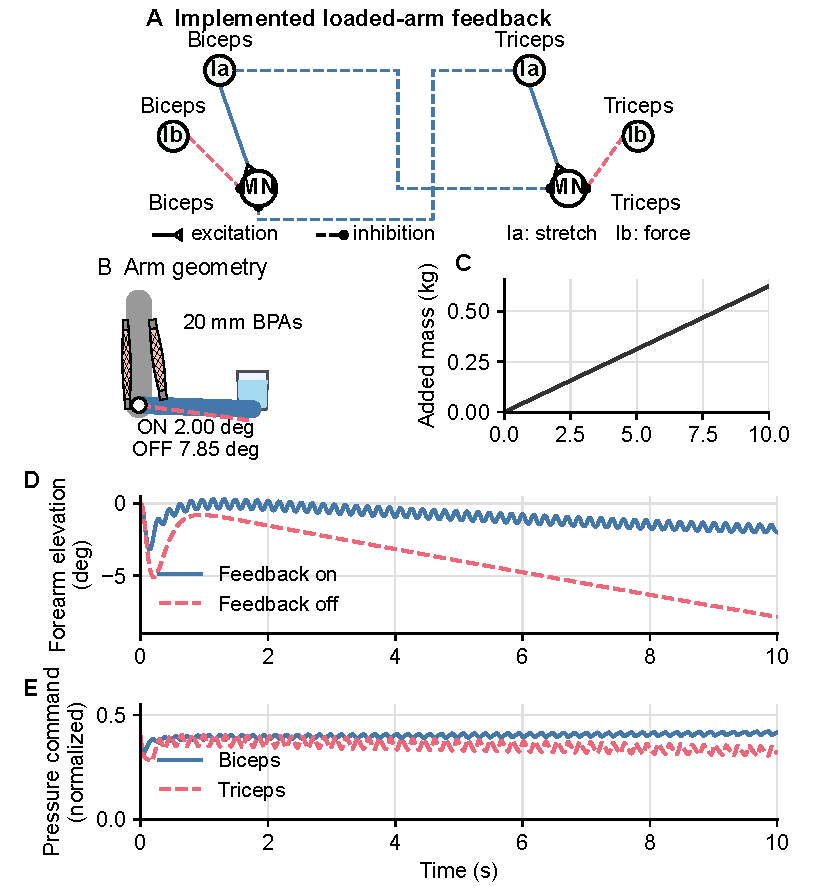
\includegraphics[width=14cm]{sns_cup_reflex_authoritative.pdf}
\caption[Loaded-cup feedback comparison]{Feedback circuit (A), arm geometry (B), load ramp (C), elevation response (D), and normalized pressure command (E). The BPA20 block supplies actuator force. The \qty{10}{\second} endpoint compares responses during increasing load, rather than equilibrium sag.}
\label{fig:sns_beverage_current}
\end{figure}
\FloatBarrier
\subsection{Staged Human-Model Experiments}\label{sec:sns_biw2l_results}

The revised graded BiW2Lvar+ controller completed both \qty{16}{\second} suspended trials with the same learned weights and PF-to-MN expression scale of 0.1. From \qty{5}{\second} to just before \qty{14}{\second}, the detector found four principal knee-flexion peaks per side in the first trial and seven in the second. The corresponding periods were \qty{2.466}{\second} and \qty{1.300}{\second}, with bilateral timing errors of 0.0337 and 0.0933 cycles from antiphase (Figure~\ref{fig:sns_biw2l_air}). The retained adapter specifies two changes between trials. It enables sensory return and raises the sustained normalized flexor and extensor commands from zero to 0.15 on both sides. The original launch adapter and complete command histories were unavailable, and the period difference cannot be assigned to feedback alone.

\begin{figure}[!htbp]
\centering
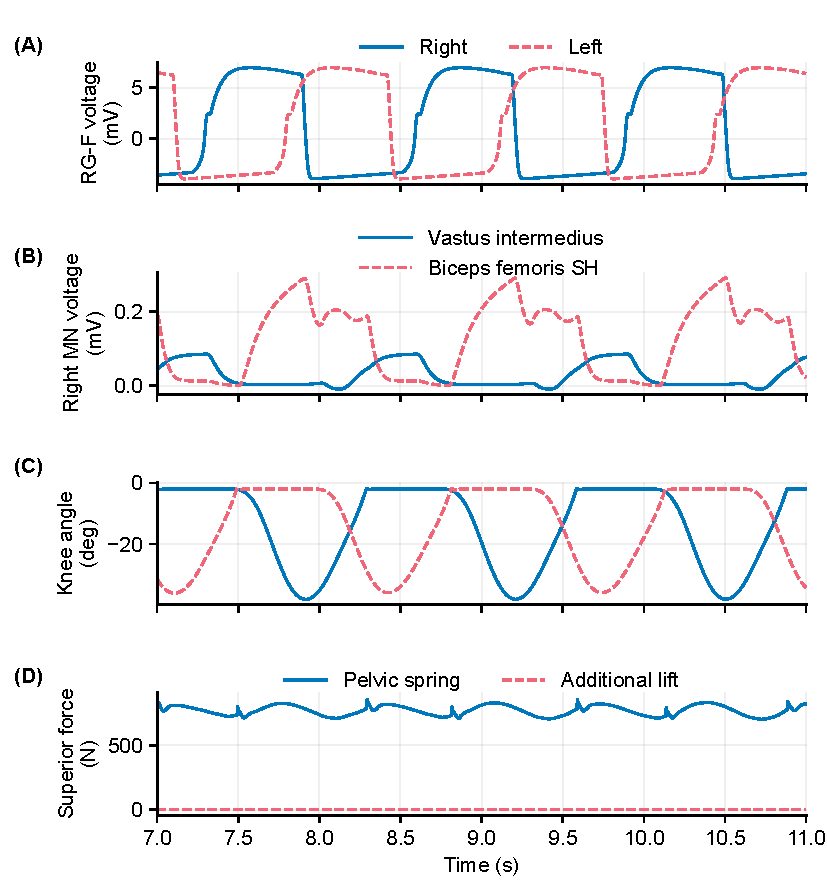
\includegraphics[width=14cm]{biw2lvar_air_aligned_authoritative.pdf}
\caption[BiW2Lvar+ afferented air-stage recording]{Aligned stage-2 signals over \qtyrange{7}{11}{\second}: bilateral flexor RG voltage (A), right knee-extensor and knee-flexor MN voltages (B), native flexion-negative knee angles (C), and superior suspension and explicit-support forces (D). Voltages are rest-relative. All saved samples are retained. Ground contact is disabled, measured foot forces are zero, and suspension and frontal guidance remain active.}
\label{fig:sns_biw2l_air}
\end{figure}

Foot forces were zero in these trials. From \qty{5}{\second} onward in the afferented condition, the suspension carried an average of \qty{99.860}{\percent} of the weight used by the original evaluator, which included a fixed ground body. Both knees remained flexed, with maximum angles of \ang{-1.718} on the right and \ang{-1.801} on the left in the model's flexion-negative convention. These trials establish suspended coordination for this controller. Appendix~\ref{sec:app_biw2l_air} gives the force numerator, weight denominator, and sampling windows.

The same candidate sustained suspended motion under continuous noise applied to RG current. All six trials, three seeds at each of two noise amplitudes, met the duration, motion, frontal-separation, and knee criteria. Repeating a seed in a fresh process reproduced the noise, neural states, and joint states. Appendix~\ref{sec:app_current_noise} specifies the noise amplitudes and correlation time.
\FloatBarrier
{\interlinepenalty=10000 The effect of a pulse depended on when it arrived. At \qty{7.10}{\second}, a \qty{2}{\nano\ampere}, \qty{100}{\milli\second} pulse changed the right hip-flexor PF voltage without reaching the outgoing synapse's transmission threshold. At \qty{7.65}{\second}, during an active phase, the same pulse changed PF voltage by up to \qty{1.14}{\milli\volt} and right iliacus MN voltage by \qty{0.16}{\milli\volt} over the \qty{3.4}{\second} following onset. Direct stimulation of the right iliacus MN also affected the RG through the closed mechanical and sensory loop (Appendix~\ref{sec:app_biw2l_stimulus}).\par}

\subsection{Controlled Interventions and Intermediate Timing Checks}\label{sec:sns_feedback_test}\label{sec:sns_literature_results}\label{sec:layer_stimulus_main}

{\interlinepenalty=10000 In a separate W2L treadmill experiment, I tested whether the fitted controller needed its sensory pathways to coordinate foot contact. I zeroed the selected sensory inputs and pathway conductances, held the remaining fitted parameters, drive, and support settings fixed, and applied the same \qty{40}{\newton} forward pulse from \qty{8}{\second} to \qty{8.15}{\second} in both runs. Median bilateral contact phase shifted from 0.498 to 0.223 cycles, outside the accepted 0.35--0.65 interval around antiphase. The model still displaced \qty{1.996}{\meter} forward over \qtyrange{4.5}{30}{\second}, compared with \qty{2.239}{\meter} with feedback (Figure~\ref{fig:sns_ablation_pair}). The pathways helped place one footfall between successive contralateral footfalls. Forward displacement alone would have missed that loss of coordination.\par}

\begin{figure}[!htbp]
\centering
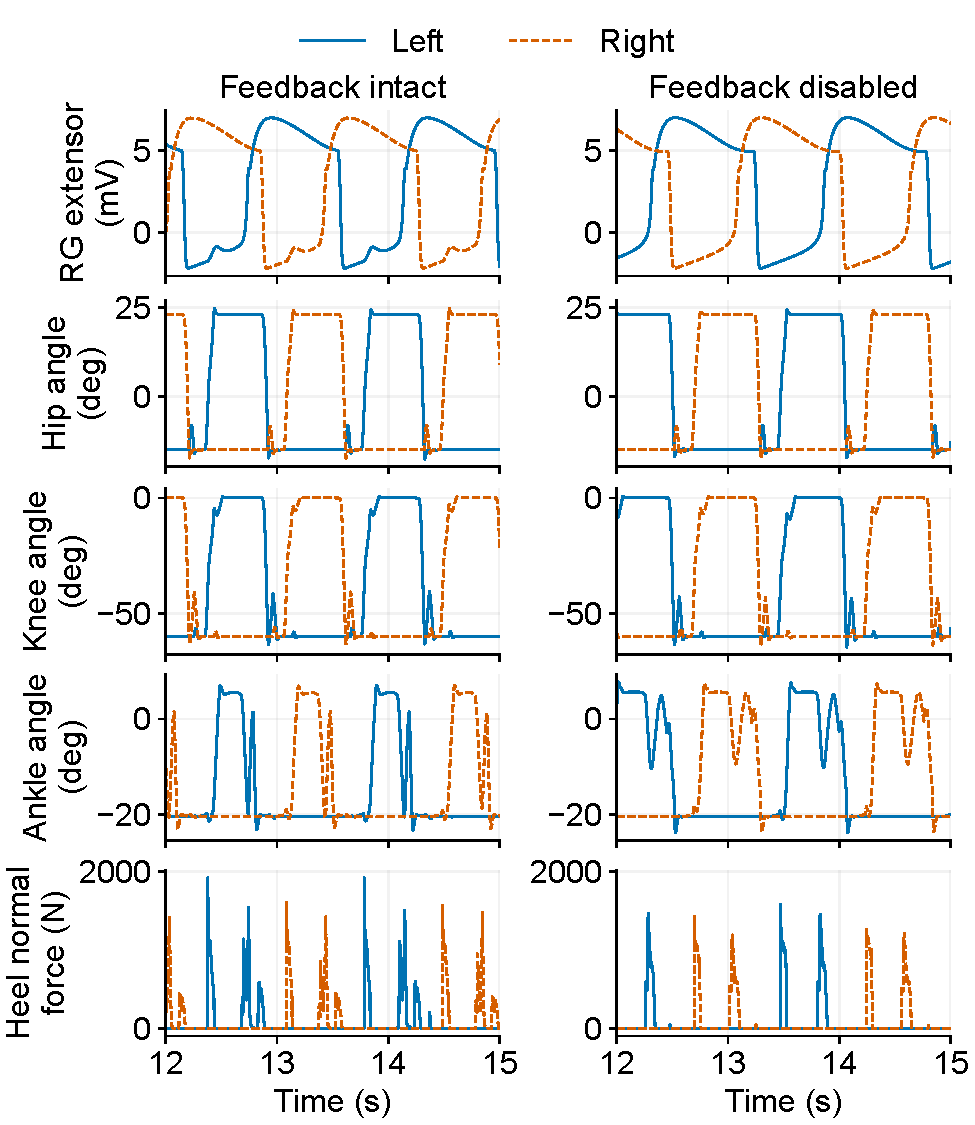
\includegraphics[width=\textwidth,height=0.74\textheight,keepaspectratio]{w2l_feedback_short_20261031.pdf}
\caption[W2L sensory-pathway removal]{RG voltages, joint angles, and heel normal forces over \qtyrange{12}{15}{\second} with sensory pathways intact (left column) and after their specified combined removal (right), at matched drive, support, and perturbation. Solid lines show the left leg and dashed lines the right. Joint cycling continued in both conditions. Bilateral contact phase was calculated over $4.5\leq t<30$\,s.}
\label{fig:sns_ablation_pair}
\end{figure}


{\interlinepenalty=10000 In the human-model controllers s3k and syn6, the fitted motor output concealed a PF timing error. In the original syn6 evaluation, none of twelve channels passed the combined timing criteria. Three components per side explained \qty{99}{\percent} of the centered variance in transmitted PF activity, compared with six components for the intended primitives. One channel remained active throughout the cycle. The corresponding s3k signals required two components per side, but that design lacked quantitative target windows against which to score individual channels.\par}

{\interlinepenalty=10000 Adjusting synaptic gains alone improved the syn6 fit without bringing any of its twelve channels within the timing criteria. RG-triggered relays and native SNS timing circuits addressed the timing directly. At nominal cadence the native circuit passed all 48 channel-cycle checks. Adaptive timing passed at six prescribed replay cadences. These checks scored individual cycles, including onset and offset, whereas the original twelve checks scored channel means. When live sensory input replaced prescribed replay, coupled trials reached the predictive knee limit or finished without meeting the rhythm and PF timing criteria. The next design question is how sensory input shifts the onset and termination of PF transmission. Appendix~\ref{sec:app_pf_timing} gives the replay and coupled-body tests.\par}

{\interlinepenalty=10000 Reduced circuits also provided physiological reference phenomena. A Rybak-derived circuit produced a missing motor burst with preserved rhythm phase in one intervention and a phase reset in another. In a Deng-derived circuit, separate RG, PF, and MN stimuli allowed the disturbance to be followed across layers \citep{rybak_modelling_2006,deng_neuromechanical_2019}. The protocols are in Sections~\ref{sec:rybak_verification} and~\ref{sec:app_layer_stimulus}.\par}

\subsection{Separate Supported-Ground Demonstrations}\label{sec:sns_ground_results}

{\interlinepenalty=10000 The W2L108 robot model, with 108 neurons and 216 connections, took eight qualifying left and seven qualifying right swings on a moving treadmill in \qty{10}{\second}. The qualifying transitions alternated, and each swing unloaded and cleared the whole foot. Minimum anatomical knee flexion over $1\leq t<10$\,s was \ang{2.087} on the right and \ang{1.946} on the left. Upward rail and guide assistance averaged \qty{29.519}{\percent} of body weight in that window. Over the complete trial, signed net assistance averaged \qty{35.069}{\percent}. An independent replay reproduced the selected trajectory. Rails, guides, and belt motion were part of the tested task.\par}

{\interlinepenalty=10000 A slower W2L108 candidate reduced upward assistance to about \qty{10.1}{\percent} over \qtyrange{2}{16}{\second} and retained seven swings per side. It missed the short-shuffle target because foot excursions were large and sustained double support was too brief (Appendix~\ref{sec:app_w2l108_ground}).\par}

{\interlinepenalty=10000 On the separately assembled CAD robot, an SNS supplied timing while an engineering controller allocated posture, loading, and clearance targets among 54 ideal reference-tension actuators (Figure~\ref{fig:ah001_supported_control}). Over $16\leq t<28$\,s, the model produced seven qualifying right and six qualifying left swings with measured vertical assistance of \qty{77.5}{\percent} of body weight. Lateral and attitude guidance remained active. Minimum knee flexion across the complete \qty{28}{\second} trial was \ang{11.20} on the right and \ang{5.10} on the left. These results test contact handover with prescribed tensile actuation. The separate BPA interface evaluates force from length and pressure.\par}

\begin{figure}[!htbp]
\centering
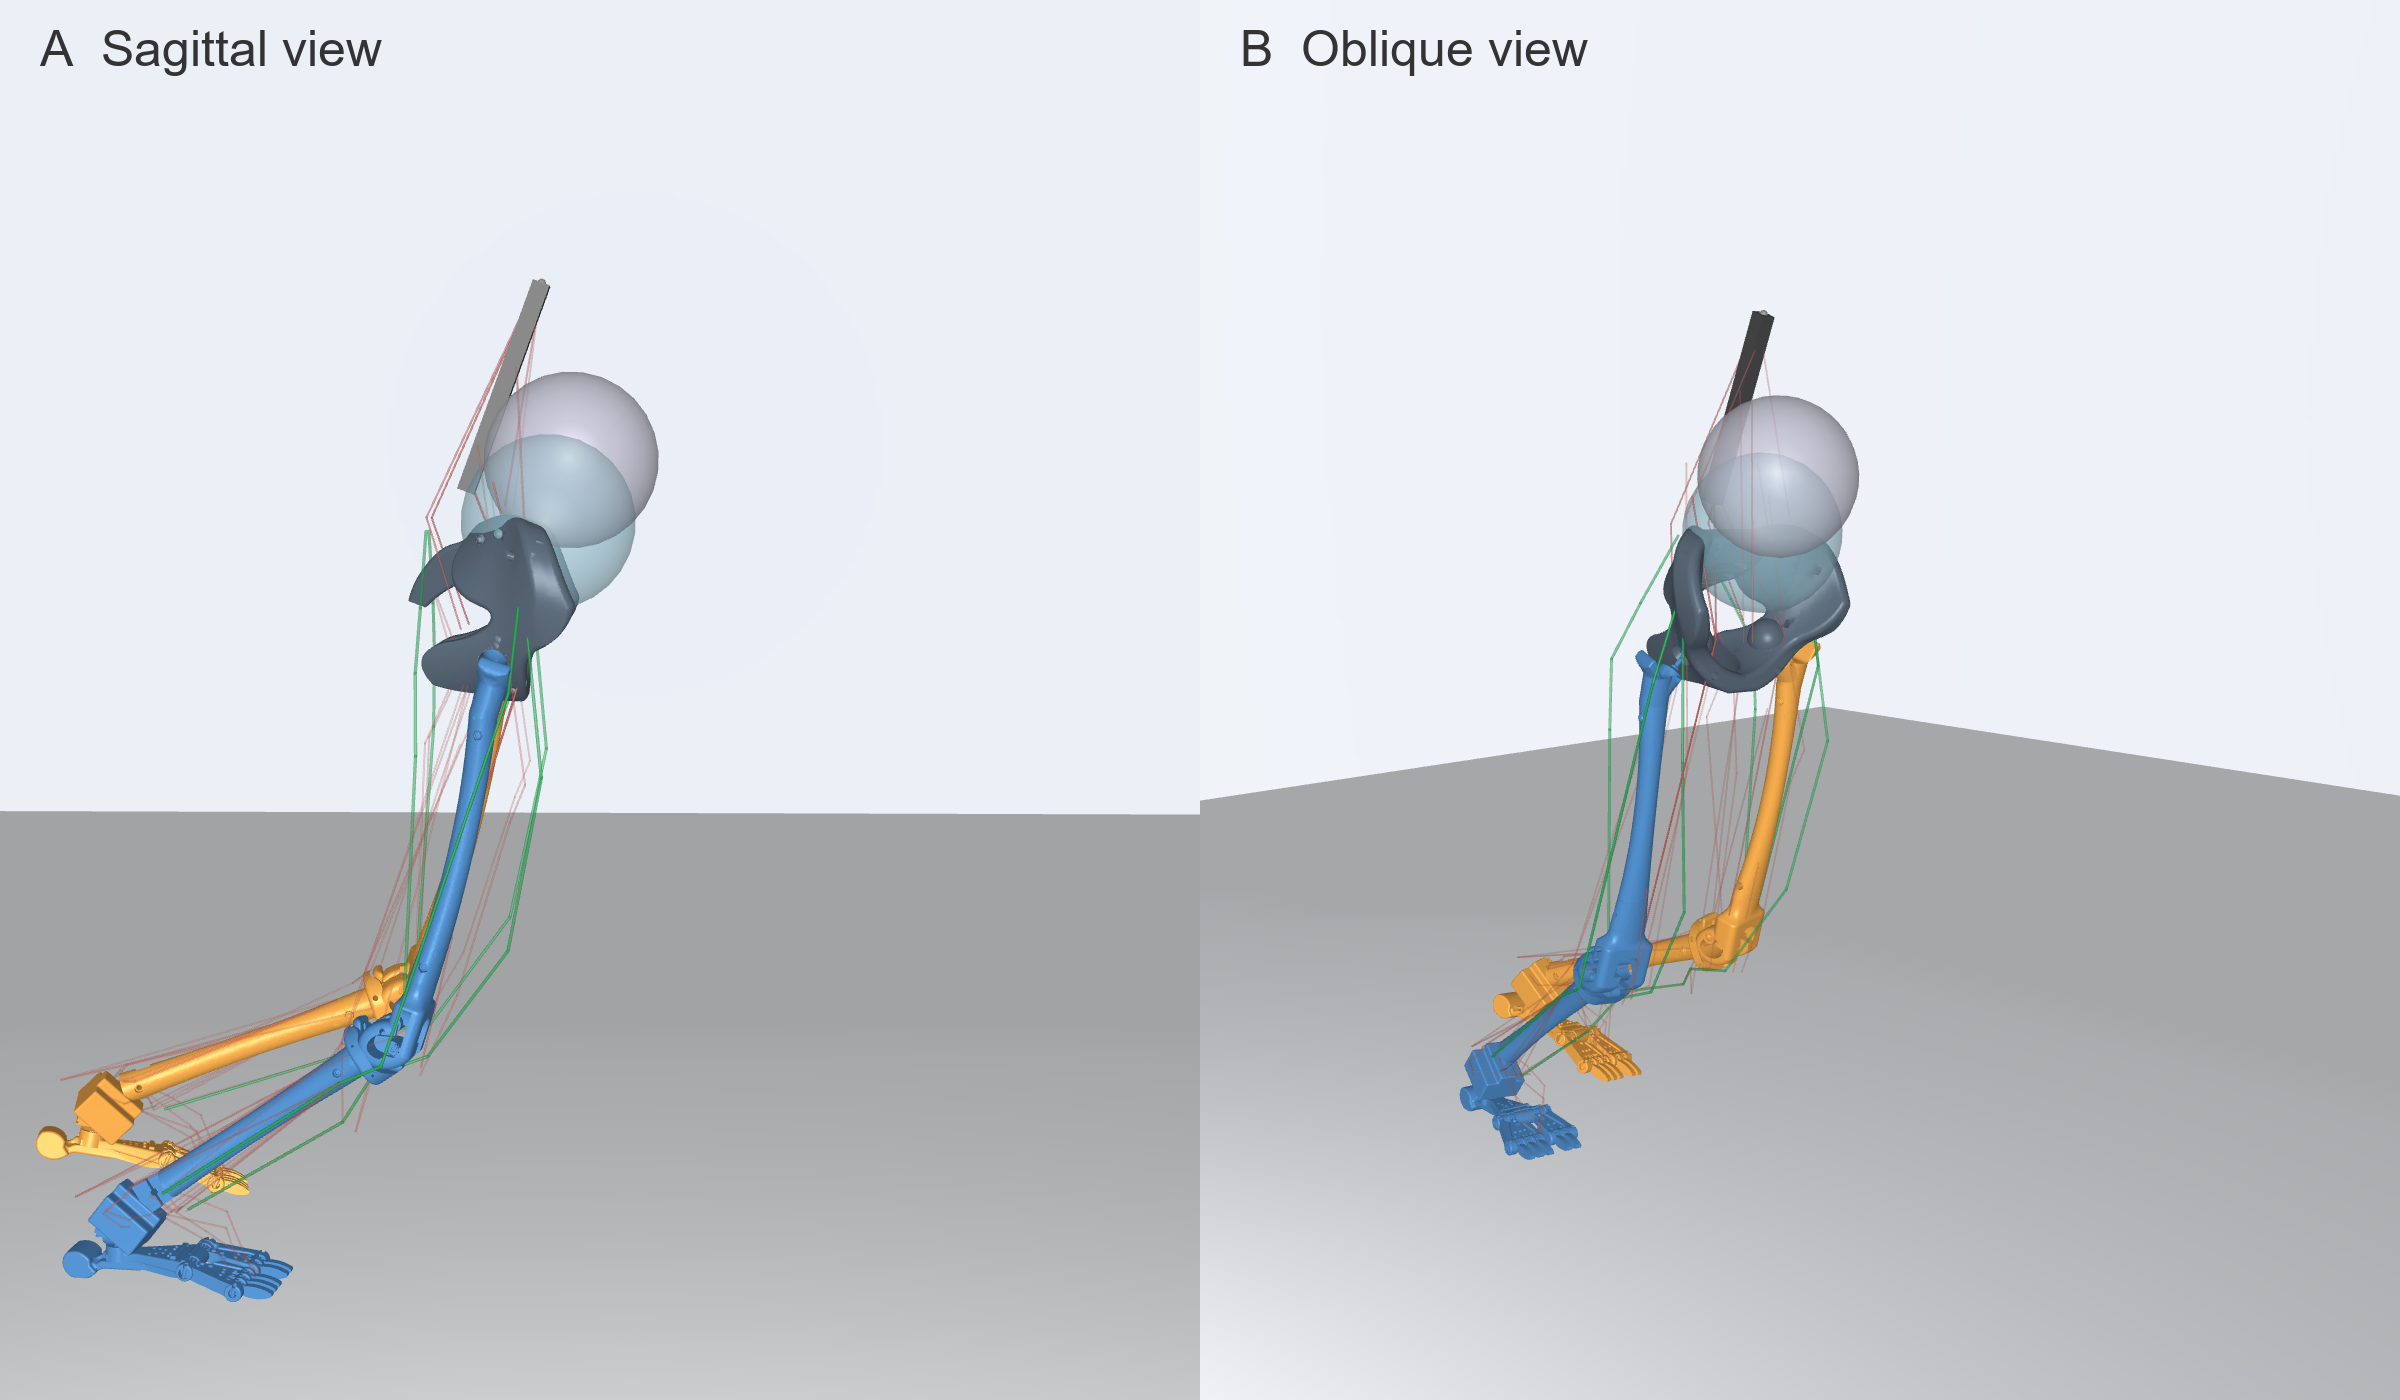
\includegraphics[width=\textwidth,height=0.48\textheight,keepaspectratio]{cad_supported_20261116.png}
\caption[CAD robot under supported hybrid control]{Views of the selected CAD robot at \qty{22.9}{\second}. The model uses 54 reference-tension actuators, SNS timing, and engineering force allocation. During \qtyrange{16}{28}{\second}, measured vertical assistance is \qty{77.5}{\percent} of body weight; lateral and attitude guidance remain active.}
\label{fig:ah001_supported_control}
\end{figure}

{\interlinepenalty=10000 The recorded CAD trajectories agreed on the reference and accelerated neural backends and in an independent repeat. Five of eight perturbations of shared controller, contact, clearance, or passive parameters finished successfully. The remaining three reached the predictive knee margin. Appendix~\ref{sec:app_cad_supported_stance} shows the loading and clearance traces.\par}

\subsection{Computational Performance}\label{sec:sns_execution}

{\interlinepenalty=10000 The sparse neural implementation stores the circuit topology once and reuses its arrays at each update. I timed it against the native SNS implementation only after matching the trajectories of the same controller and body. In one paired \qty{16}{\second} Gait2392 stage-1 trial using the 1,025-cell \texttt{hunt} source configuration, the complete external process took \qty{199.624}{\second} with native SNS and \qty{29.284}{\second} with the sparse backend. This measures a $6.82\times$ speedup for the process, including \qty{0.6}{\second} of simulated held-pose preparation. Timing just the neural calls within that pair gave $18.31\times$ (Table~\ref{tab:sns_runtime}).\par}

\begin{table}[htbp]
\centering\small
\caption[Scoped computational performance comparisons]{Matched reference and accelerated timings. The first two rows use the 1,025-cell source-setting \texttt{hunt} implementation, native SNS versus sparse execution, in one \qty{16}{\second} stage-1 protocol pair. The last two use the separate 1,033-cell implementation labelled Hunt-PT+RC, sparse versus compact execution. Warm-kernel values are medians of three blocks; the evaluator diagnostic is one paired \qty{16}{\second} stage-4 trial.}
\label{tab:sns_runtime}
\begin{tabularx}{\textwidth}{@{}>{\raggedright\arraybackslash}Xrrr@{}}
\toprule
Measured computation & Reference (s) & Accelerated (s) & Ratio \\
\midrule
Gait2392 complete source process & 199.624 & 29.284 & $6.82\times$ \\
Same trial, neural-call portion & 179.079 & 9.780 & $18.31\times$ \\
Compact comparison, 3,000 warm neural updates & 0.895287 & 0.555062 & $1.613\times$ \\
Compact comparison, evaluator diagnostic wall time & 92.944 & 91.516 & $1.0156\times$ \\
\bottomrule
\end{tabularx}
\end{table}

{\interlinepenalty=10000 For the 1,033-cell Hunt-PT+RC controller, the compact backend reproduced all 62 captured arrays and the compiled model identity. Its warm neural timing was the median of three blocks of 3,000 updates. The separate \qty{16}{\second} stage-4 diagnostic timed the coupled evaluator, recording, and assessment. The timer excluded process startup, pre-run setup, and final serialization. Improving the neural calculation by $1.613\times$ improved that evaluator time by only $1.0156\times$. This difference matters when estimating how many complete trials a parameter search can run (Appendix~\ref{sec:app_execution_provenance}).\par}

\section{Discussion}\label{sec:sns_discussion}

\subsection{What Can Be Transferred Between Models}

A muscle-force comparison can identify a mechanical discrepancy before neural parameters are adjusted. The knee and cup experiments then show what changes when sensory current reaches a motor pool in a model whose load and actuator law are known. By the time a foot touches the treadmill, the same comparison requires a record of contact, actuator force, and external assistance. The progression from one joint to a supported biped makes it possible to ask which part of the loop accounts for a change in behavior.

The W2L sensory intervention illustrates the value of separate outcome measures. The model moved forward under both conditions, although contact timing fell outside the accepted range after the combined removal. In syn6, the opposite problem arose during fitting. An acceptable pattern of motor recruitment concealed a PF channel that remained active throughout the cycle. Recording the signal at the receiving layer distinguished a successful output fit from a circuit that performed its intended function.

\subsection{Interpreting Sensory and Mechanical Support}

The human drive-weaning experiment separated a particular descending input from the mechanical assistance. The human model continued to step in place under its support rig when supplementary left and right drive reached zero. The shared descending input remained active. In a separate W2L robot experiment the model progressed with reduced supplementary drive while the harness remained engaged (Appendix~\ref{sec:sns_controller_comparison}).

Suspension removes ground loading. Rails and guides permit contact but carry part of the weight and constrain motion. The evidence for the BiW2Lvar+ air stages, the W2L pathway removal, W2L108 treadmill stepping, and the CAD model's contact handover therefore applies to four distinct experimental conditions. No experiment in this program established harness-free walking.

The force law also determines what a controller test can establish. The simplified knee actuator isolates the response to a sensory pulse. The BPA20 arm model tests whether the feedback circuit can recruit enough pressure-dependent force as a load increases. Specifying ideal tensions on the CAD model isolates the demands of contact and swing clearance. Applying its controller to physical BPAs introduces a further question about attainable force at each measured length and pressure.

\subsection{Opportunities for Further Integration}

The syn6 result motivates a specific transfer experiment. Record the same PF channel first under prescribed sensory input and then during closed-loop motion. Compare the timing of transmitted output and the knee state when the two responses diverge. This would distinguish a failure of the neural timing circuit under altered input from a mechanical limit that a well-timed command cannot avoid.

For a muscle with poor matched-pose force agreement, a comparison across prescribed movement velocities could separate effects of tendon compliance and activation history. For the robot model, the corresponding experiment would apply a measured pressure history to a characterized BPA route. Repeating a contact or controller test on the repaired model would then show whether the mechanical change affected coordination.

The embedded interface provides a starting point for a hardware test. Its sensory encoding, command exchange, and watchdog can be exercised with recorded signals before connecting valves. The compiled SNS binding and physical I/O still require integration (Appendix~\ref{sec:app_embedded_interfaces}). Chapter~\ref{ch:overall} relates this test to the actuator and knee measurements.

\section{Chapter Conclusion}

I developed a way to carry a controller from a circuit diagram to a mechanical test with an identifiable input and output. A colleague can repeat the sensory pulse at the knee, disable a pathway on a supported walker, or compare the timing of a PF signal before and after closing the loop. The task, actuator law, and assistance determine which conclusions each of those experiments supports.

\widowpenalty=\snsSavedWidowPenalty\relax
\clubpenalty=\snsSavedClubPenalty\relax
